5. Al evaluar una integral doble sobre una región \( D \) se obtuvo una suma de integrales iteradas como sigue:
\[
\iint_{D} f(x, y) d A=\int_{0}^{1} \int_{0}^{2 y} f(x, y) d x d y+\int_{1}^{3} \int_{0}^{3-y} f(x, y) d x d y
\]

Describa la región \( D \) y exprese la integral doble como una integral iterada con el OTRO orden de integración. Finalmente dibuje la región \( D \). \\

Analicemos los límites de integración en cada término:  

Para la primera integral reunimos las siguientes características.
\begin{itemize}
    \item \( y \) varía de \( 0 \) a \( 1 \).
   \item Para cada \( y \), \( x \) varía de \( 0 \) a \( 2y \).
\end{itemize}

Para la segunda.
\begin{itemize}
    \item \( y \) varía de \( 1 \) a \( 3 \).
   \item Para cada \( y \), \( x \) varía de \( 0 \) a \( 3 - y \).
\end{itemize}

Combinando ambas partes, la región \( D \) es:

\[
D = \{(x,y) \in \mathbb{R}^2 \mid 0 \leq x \leq 3, 0 \leq y \leq g(x)\},
\]

donde \( g(x) \) es la frontera superior de \( y \) en términos de \( x \); vease que para \( 0 \leq x \leq 2 \), despejamos \( y \) de \( x \leq 2y \):  
  \[
  y \geq \frac{x}{2}.
  \]
  Ahora para \( 2 \leq x \leq 3 \), despejamos \( y \) de \( x \leq 3 - y \):  
  \[
  y \leq 3 - x.
  \]

Por lo tanto, la región \( D \) está acotada por \( x \) en \( [0,3] \), y por \( y \) en:

\[
\frac{x}{2} \leq y \leq 3 - x.
\]

El orden actual es \( dy \) externo y \( dx \) interno. Para cambiar el orden, describimos \( D \) en términos de \( x \) como variable externa, obsérvese que \( x \) varía entre \( 0 \) y \( 3 \), además para cada \( x \), \( y \) varía entre \( \frac{x}{2} \) y \( 3 - x \). \\

La nueva integral es:

\[
\iint_D f(x,y) dA = \int_0^3 \int_{\frac{x}{2}}^{3-x} f(x,y) \,dy\,dx.
\]

Miremos que la recta \( x = 2y \) pasa por \( (0,0) \) y \( (2,1) \); la recta \( x = 3 - y \) pasa por \( (3,0) \) y \( (0,3) \); la región está delimitada por estas curvas en \( 0 \leq x \leq 3 \). Esto nos denota 3 intersecciones expresadas como un triángulo con vértices en \( (0,0) \), \( (2,1) \) y \( (3,0) \).

\begin{figure}[h]
    \centering
    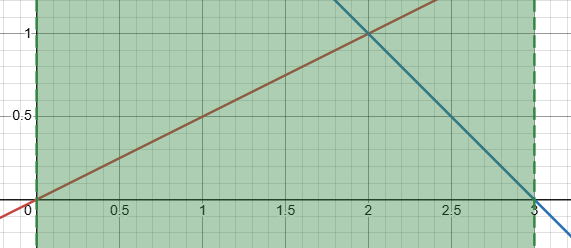
\includegraphics[width=0.5\linewidth]{triangle5.png}
    \caption{Región descrita en el Ejercicio V}
    \label{fig:enter-label}
\end{figure}